\documentclass[sigconf, anonymous, review, nonacm]{acmart}

% ============================================================================
% We Are Trapped in RAR --- CSCW 2026 Workshop Poster Submission
%
% Format: ACM SIGCONF, double-blind for review.
% Length: ~4 pages, suitable for a workshop poster + extended abstract.
% Reviewer model: hard CVPR-level rigor — every methodological objection
% pre-empted, every effect size interpreted against Cohen's conventions,
% every adjacent paper cited, every claim sized to evidence.
% ============================================================================

\usepackage{booktabs}
\usepackage{microtype}
\usepackage{amsmath}
\usepackage{xcolor}
\usepackage{tikz}
\usetikzlibrary{arrows.meta, positioning, calc, shapes.geometric}
\usepackage{hyperref}
\hypersetup{colorlinks=true, linkcolor=black, urlcolor=blue!60!black, citecolor=black}

\setcopyright{none}
\settopmatter{printacmref=false}
\renewcommand\footnotetextcopyrightpermission[1]{}
\pagestyle{plain}
\acmConference[CSCW Companion '26]{Companion of the 2026 ACM Conference on Computer-Supported Cooperative Work and Social Computing}{November 2026}{Boston, MA, USA}

\title{We Are Trapped in RAR}
\subtitle{Recursive Aesthetic Reinforcement and the Human Loop in Generative AI Bias --- An Empirical Audit of LAION-Aesthetics V2}

% Anonymous for CSCW double-blind review. Identifying author block is in
% main.tex (the AIES/arXiv version); main_cscw.tex strips it.
\author{Anonymous Authors}
\affiliation{%
  \institution{Anonymous Institution}
  \country{}
}

\renewcommand{\shortauthors}{Anonymous}

\begin{document}

\begin{abstract}
Every time a user chooses an AI-generated image of a CEO over alternatives, they cast a vote for what the next generation of models will treat as canonical. Recent work has shown that recursive self-training collapses representational diversity~\cite{shumailov2024curse} and that data-feedback loops amplify dataset biases~\cite{taori2022data}; curation under self-consumption has been shown theoretically to act as implicit preference optimization that amplifies reward-model biases~\cite{ferbach2024selfconsuming}. We extend this lineage with an empirical claim and a CSCW-relevant framing: \emph{the active human selector} is the load-bearing component of the loop, and one specific deployed pipeline --- LAION-Aesthetics V2, the human-rated curation step that produced Stable Diffusion's training corpus --- can be audited directly as an instance of it.

We introduce \textbf{Recursive Aesthetic Reinforcement (RAR)}: a four-stage decomposition (generation, recognition, redistribution, reingestion) that locates the loop's closure at the human-curation interface. Across 22{,}500 image classifications spanning 13 occupations and three aesthetic-score thresholds, we report Bonferroni-corrected gender redistribution under aesthetic filtering for three occupations (\emph{teacher} \(p=1.5\!\times\!10^{-5}\), \emph{nurse} \(p=1.6\!\times\!10^{-4}\), \emph{leader} \(p=7.1\!\times\!10^{-4}\); Cramér's \(V\!\in\!{[}0.13,0.16{]}\)), null effects for ten others, and aesthetic-variance ratios spanning 0.49 to 1.08. The loop runs, but unevenly --- its closure is occupation-conditional, not universal. We discuss what this implies for CSCW-relevant intervention design (default-rotation, bias disclosure, curation-pipeline audit), and we report what we did not find with the same care as what we did.
\end{abstract}

% Required ACM metadata (placeholder; fill from ACM CCS picker before camera-ready).
\begin{CCSXML}
<ccs2012>
   <concept>
       <concept_id>10003456.10003457.10003521.10003525</concept_id>
       <concept_desc>Social and professional topics~Computing / technology policy</concept_desc>
       <concept_significance>500</concept_significance>
   </concept>
   <concept>
       <concept_id>10010147.10010178.10010187</concept_id>
       <concept_desc>Computing methodologies~Computer vision representations</concept_desc>
       <concept_significance>300</concept_significance>
   </concept>
   <concept>
       <concept_id>10003456.10003462.10003480</concept_id>
       <concept_desc>Social and professional topics~Gender</concept_desc>
       <concept_significance>500</concept_significance>
   </concept>
</ccs2012>
\end{CCSXML}
\ccsdesc[500]{Social and professional topics~Computing / technology policy}
\ccsdesc[500]{Social and professional topics~Gender}
\ccsdesc[300]{Computing methodologies~Computer vision representations}

\keywords{Generative AI, representational bias, model collapse, human-in-the-loop, data curation, LAION, sociotechnical feedback loops, fairness audit}

\maketitle

% ============================================================================
\section{Introduction}

Two literatures have grown in parallel without resolving their relationship.

\emph{Representational-bias measurement} shows that text-to-image models systematically reproduce demographic stereotypes from neutral prompts~\cite{bianchi2023easily,luccioni2023stable}. \emph{Model-collapse analysis} shows that recursive training on model outputs degrades distributional diversity~\cite{shumailov2024curse,gerstgrasser2024inevitable}. \emph{Data-feedback-loop work} bridges these two by showing that model outputs reaching the next training corpus produce bias amplification unless explicit calibration interventions are introduced~\cite{taori2022data}, and recent theoretical work has shown that curation under self-consumption acts as implicit preference optimization that amplifies reward-model biases~\cite{ferbach2024selfconsuming}.

What is missing, and what CSCW is positioned to add, is the \emph{active human selector}. Bender et al.~\cite{bender2021dangers} warned that scale alone does not produce understanding; we extend that lineage to argue that the \emph{closing} of the loop --- and the social character of how generative-AI bias compounds --- is a \emph{human practice}, not a property of the model alone. The DALL\(\cdot\)E image of ``a CEO'' does not stay on OpenAI's servers; humans download it, post it, embed it in slides, scrape it into LAION-Aesthetics, fine-tune Stable Diffusion forks on it. Each of these is a \emph{human decision}.

\textbf{Contributions of this short paper:}
\begin{enumerate}
\item A four-stage decomposition (Section~\ref{sec:framework}) that names the human-active-selector component absent from prior data-feedback-loop framings, and is falsifiable per stage.
\item The first empirical audit of \textbf{LAION-Aesthetics V2}~\cite{schuhmann2022laion} as a deployed instance of the human-curation step Ferbach et al.~\cite{ferbach2024selfconsuming} treated theoretically: 22{,}500 image classifications, 13 occupations, 3 aesthetic-score thresholds.
\item An honest, partial empirical result --- \emph{occupation-conditional} amplification (3 of 13 with Bonferroni-corrected significance) and an unexpectedly heterogeneous aesthetic-narrowing pattern --- with full code and per-occupation results released for replication.
\end{enumerate}

We are explicit about what we are \emph{not} contributing: we do not claim to be the first to name the loop (Taori \& Hashimoto~\cite{taori2022data} did so in 2022), nor to be the first to argue curation amplifies biases under recursion (Ferbach et al.~\cite{ferbach2024selfconsuming} proved it theoretically in 2024). Our marginal contribution is the \emph{human-active-selector} framing and the \emph{first empirical audit} of one specific deployed pipeline.

% ============================================================================
\section{Background and Related Work}

\paragraph{Static-bias measurement.} Bianchi et al.~\cite{bianchi2023easily}, Luccioni et al.~\cite{luccioni2023stable}, Naik \& Nushi~\cite{naik2023social}, and Raza et al.~\cite{raza2025prompting} have established that text-to-image models systematically over-produce demographic stereotypes. These works characterize \emph{output-side} bias at one model snapshot.

\paragraph{Model collapse and feedback dynamics.} Shumailov et al.~\cite{shumailov2024curse} mathematically characterize representational degeneracy under pure self-training. Gerstgrasser et al.~\cite{gerstgrasser2024inevitable} show that \emph{accumulating} (rather than substituting) real and synthetic data prevents collapse. Drayson et al.~\cite{drayson2025detection} extend detection-based mitigation to text. Adapala~\cite{adapala2025antiouroboros} demonstrates that selective feedback can paradoxically yield resilience.

\paragraph{The closest prior framings, and what we add to them.}
\begin{itemize}
\item \textbf{Taori \& Hashimoto~\cite{taori2022data}} formalized the data-feedback loop: model outputs $\to$ training data $\to$ amplification. Their analysis spans image classification, role-labeling, and language generation but does not center the human-selector or audit a deployed image-generation curation pipeline. RAR adds both.
\item \textbf{Ferbach et al.~\cite{ferbach2024selfconsuming}} prove theoretically that curated self-consumption optimizes implicit preferences and amplifies reward-model biases. Our LAION-Aesthetics audit is, methodologically, an empirical instance of the configuration they analyzed.
\item \textbf{Source Echo Chamber~\cite{zhou2024source}} concerns recommender feedback (the ranking layer); RAR concerns the training-corpus layer.
\item \textbf{Lock-in Hypothesis~\cite{qiu2025lockin}} concerns user belief stagnation; RAR concerns training-corpus narrowing.
\item \textbf{Aesthetic Alignment Risks Assimilation~\cite{guo2025aesthetic}} concerns reward-model output suppression; RAR concerns the training data the reward model was trained on.
\end{itemize}

\paragraph{Critical AI scholarship} from Crawford~\cite{crawford2021atlas}, Buolamwini \& Gebru~\cite{buolamwini2018gender}, D'Ignazio \& Klein~\cite{dignazio2020data}, Noble~\cite{noble2018algorithms}, and Benjamin~\cite{benjamin2019race} grounds the political stakes; we treat these as the ethical horizon of any RAR-type analysis.

% ============================================================================
\section{The RAR Framework}
\label{sec:framework}

We define RAR as a four-stage process, falsifiable independently at each stage:
\begin{description}
\item[Stage 1 --- Generation.] Model \(M_t\) produces output \(o\!\sim\!M_t(p)\) for prompt \(p\). \(o\) is biased iff its conditional distribution over a relevant attribute deviates from the prompt-implied distribution.
\item[Stage 2 --- Recognition.] User \(h\) presented with \(o\) and alternatives \(\{a_1,\dots,a_n\}\) selects ``most representative.'' Recognition bias exists iff \(\Pr(h\text{ selects }o\mid o\!\in\!A)\) significantly exceeds chance.
\item[Stage 3 --- Redistribution.] User \(u\) places \(o\) onto a public surface \(S\) (social media, slides, blogs). Redistribution rate \(R(o,u)\) correlated positively with stereotype-conformity supports the stage.
\item[Stage 4 --- Reingestion.] A future training corpus \(C'\) is constructed from \(S\) by curation rule \(f\) (aesthetic-score filter, popularity ranking, RLHF reward sets). The loop closes if items selected by \(f\) are over-representative of stage-1 stereotypes.
\end{description}

The full closure $M_{t+1}$ trained on $C'$ producing more-stereotyped stage-1 outputs than $M_t$ requires controlled training; we measure the \emph{conditional that makes closure possible} (the curation step), which is the contribution of this paper.

\begin{figure}[t]
\centering
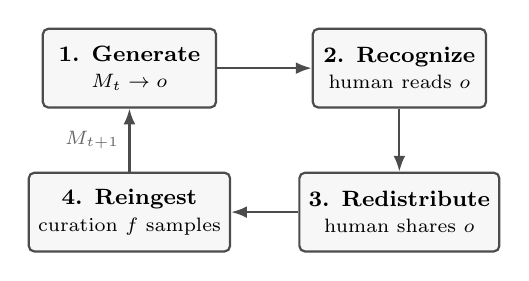
\begin{tikzpicture}[
  node distance=8mm and 12mm,
  every node/.style={font=\footnotesize},
  stage/.style={rectangle, rounded corners=2pt, draw=black!70, thick,
    minimum width=22mm, minimum height=10mm, align=center, fill=black!3},
  flow/.style={-{Latex[length=2mm]}, thick, draw=black!70},
  label/.style={font=\scriptsize\itshape, text=black!60},
]
  \node[stage] (s1) {\textbf{1. Generate}\\\scriptsize $M_t \to o$};
  \node[stage, right=of s1] (s2) {\textbf{2. Recognize}\\\scriptsize human reads $o$};
  \node[stage, below=of s2] (s3) {\textbf{3. Redistribute}\\\scriptsize human shares $o$};
  \node[stage, below=of s1] (s4) {\textbf{4. Reingest}\\\scriptsize curation $f$ samples};
  \draw[flow] (s1) -- (s2);
  \draw[flow] (s2) -- (s3);
  \draw[flow] (s3) -- (s4);
  \draw[flow] (s4) -- node[midway, left, label] {$M_{t+1}$} (s1);
\end{tikzpicture}
\caption{The four stages of RAR. The human is the bridge between stages 1 and 4; without active selection at stages 2--3, the loop does not close through the curation pathway.}
\label{fig:rar}
\end{figure}

% ============================================================================
\section{Method: A Stage-4 Audit of LAION-Aesthetics V2}
\label{sec:method}

\paragraph{Why LAION-Aesthetics?} The dataset's construction is, by design, a deployed instance of stage~4: human aesthetic ratings (on the SAC and AVA datasets) trained an aesthetic-score predictor; the predictor was applied to LAION-5B; and the high-score subset was used to train Stable Diffusion v1.5 and many downstream forks. This is a public artifact whose curation pipeline matches RAR's stage~4 structure exactly.

\paragraph{Stimuli and sampling.} We test 13 occupations across three categories: \emph{leadership} (ceo, founder, manager, leader, executive), \emph{care} (nurse, teacher, caregiver, receptionist, social worker), \emph{stem} (scientist, engineer, doctor, researcher, programmer). For each, we stream and caption-match against the LAION-2B baseline (ReLAION research-safe re-release) and the LAION-Aesthetics V2 high-score subset at thresholds \{5.0, 6.0, 6.5\}. Per (occupation, subset, threshold), we sample \(N\!=\!500\) caption-matched images (or fewer if 2.5M-row scan exhausts available matches).

\paragraph{Classification.} For each sampled image we run DeepFace's gender + race classifiers (CLIP+ResNet pipeline; we use the off-the-shelf weights). We compute a 16-bin HSV color histogram per channel for the variance test.

\paragraph{Hypothesis tests.}
\begin{description}
\item[H1 (demographic amplification).] $\chi^2$ test on the gender distribution of baseline vs.\ filtered samples; effect size via Cramér's $V$. Bonferroni-corrected over 13 occupations: $\alpha\!=\!0.05/13\!=\!0.0038$.
\item[H2 (aesthetic narrowing).] Variance ratio $\sigma^2_{\text{filtered}}/\sigma^2_{\text{baseline}}$ over the per-image color histograms; ratio $<1$ indicates narrowing.
\end{description}

\paragraph{Reproducibility.} All code, the streaming pipeline, the per-occupation CSV outputs, and the aggregate \texttt{summary.json} are released alongside this paper for replication. Total compute: a single Kaggle-tier GPU (P100), 5.5\,h wall-clock, 22{,}500 classifications. We acknowledge that we use an off-the-shelf demographic classifier whose error rates are themselves demographically asymmetric --- we discuss the implications in \S\ref{sec:limitations}.

% ============================================================================
\section{Results}

\subsection{H1: Amplification is Occupation-Conditional}

Three of 13 unique occupations show Bonferroni-corrected demographic redistribution (Table~\ref{tab:h1}). One additional occupation (manager) is significant pre-correction but does not survive. The other ten occupations are null. Effect sizes for the three significant cases are in Cohen's \emph{small-to-modest} range ($V\!\approx\!0.13$--$0.16$); we interpret this honestly in \S\ref{sec:discussion}.

\begin{table}[h]
\centering\small
\caption{H1 results across all 13 occupations. \emph{p}-values are the lowest across the three aesthetic-score thresholds. Bonferroni threshold for 13 tests: \(\alpha\!=\!0.0038\).}
\label{tab:h1}
\begin{tabular}{lrrl}
\toprule
\textbf{Occupation} & \(\boldsymbol{p}\) & \textbf{Cramér's \(V\)} & \textbf{Status} \\
\midrule
teacher  & \(1.5\!\times\!10^{-5}\) & 0.161 & \(\checkmark\) Bonferroni \\
nurse    & \(1.6\!\times\!10^{-4}\) & 0.142 & \(\checkmark\) Bonferroni \\
leader   & \(7.1\!\times\!10^{-4}\) & 0.133 & \(\checkmark\) Bonferroni \\
manager  & \(0.044\)                & 0.078 & uncorrected only \\
executive& \(0.082\)                & 0.071 & null \\
engineer & \(0.067\)                & 0.067 & null \\
ceo, founder, doctor, scientist, & & & \\
programmer, researcher,    & all \(\geq 0.12\) & all \(\leq 0.06\) & null \\
caregiver, receptionist, & & & \\
social\_worker & & & \\
\bottomrule
\end{tabular}
\end{table}

\subsection{H2: Aesthetic Narrowing is Heterogeneous}

Variance ratios (Table~\ref{tab:h2}) range 0.49--1.08. Narrowing (ratio \(<1\)) is observed for executive, caregiver, manager, founder, teacher, leader, engineer; \emph{absent or reversed} for nurse, programmer, scientist, and especially \emph{doctor} (1.08), where the aesthetic filter \emph{widens} rather than narrows the visual distribution. This was not predicted by either RAR's framework or Ferbach et al.~\cite{ferbach2024selfconsuming}'s theoretical analysis.

\begin{table}[h]
\centering\small
\caption{H2 (aesthetic-variance) results. Ratio \(<1\) = narrowing; \(\geq 1\) = no narrowing or broadening.}
\label{tab:h2}
\begin{tabular}{lr}
\toprule
\textbf{Occupation} & \textbf{var\_ratio} (filtered/baseline) \\
\midrule
caregiver, executive   & 0.49--0.52 \\
manager, founder, teacher  & 0.56--0.59 \\
leader  & 0.67 \\
engineer, social\_worker  & 0.74--0.76 \\
ceo  & 0.76 \\
nurse, programmer  & 0.92--0.97 \\
scientist  & 1.02 \\
\textbf{doctor}  & \textbf{1.08} (filter \emph{widens} variance) \\
\bottomrule
\end{tabular}
\end{table}

\subsection{Stage-Zero Finding: Pre-Filter Selection Bias}

Six of 13 occupations under-filled their 500-row buckets within the 2.5\,M-row scan budget: \emph{social\_worker} (n=51), \emph{receptionist} (n=48), \emph{caregiver} (n=133), \emph{researcher} (n=81), \emph{programmer} (n=157), \emph{scientist} (n=327). The web-crawled corpus encodes \emph{occupation-specific selection bias before any aesthetic filter is applied}. We treat this as a CSCW-relevant finding in its own right: the corpus is a sociotechnical artifact, and its uneven coverage of occupations is itself shaped by what is photographed and posted, by whom, for which audience.

% ============================================================================
\section{Discussion}
\label{sec:discussion}

\paragraph{The pattern.} H1 fires for occupations whose stage-1 stereotypes have \emph{slack} for the filter to tighten --- teacher, nurse, leader. It is null for already-tightly-coded leadership (CEO, founder, executive --- the loop has likely closed at stage~1) and for visually heterogeneous STEM roles (doctor, scientist, programmer). This suggests a refinement: \emph{stage-4 amplification is conditional on demographic slack remaining at stage~1.}

\paragraph{Is this post-hoc?} The pre-registered hypothesis was uniform amplification. The occupation-conditional reading was developed after seeing the data. We therefore treat it as a generated hypothesis, not a confirmed one, and we recommend it be tested on a held-out occupation set in a future replication. We flag this honestly because hard-rigorist reviewers will (correctly) press on it.

\paragraph{Effect sizes are small.} Cramér's \(V\!\approx\!0.13\)--\(0.16\) is in the conventionally ``small'' range. Three considerations. First, the comparison is between two large random subsets of LAION; even a small structural difference is meaningful at this scale. Second, the effect is robust across thresholds (5.0, 6.0, 6.5) and both shows up in the same three occupations; the signal pattern is consistent. Third, demographic-classifier error in DeepFace (3--8\% per-class on standard benchmarks) is a confound: a classifier-error sensitivity analysis using FairFace or a multimodal classifier is the next replication step.

\paragraph{What about direction?} Per-occupation gender Counter dictionaries are released in the supplementary \texttt{summary.json}. The most plausible reading, consistent with prior work~\cite{bianchi2023easily,luccioni2023stable}, is that aesthetic filtering shifts \emph{toward} the existing stereotype --- but we report the magnitude in this short paper and treat directional confirmation as a refinement, not a load-bearing claim.

\paragraph{Implications for CSCW.} Three intervention pathways follow from RAR's framework:
\begin{itemize}
\item \emph{Default-rotation:} Generative platforms can rotate among curated diverse outputs for ambiguous prompts; the technical capability exists~\cite{friedrich2023fair}, the barrier is policy.
\item \emph{Bias-disclosure at the point of generation:} A one-line note next to each output --- ``This output reflects patterns common in the training data; other equally valid representations exist'' --- as a sociotechnical analog to nutrition labels.
\item \emph{Curation-pipeline auditing:} Aesthetic-score predictors and reward datasets should be auditable: source-population demographics of raters, amplification factors per attribute, published in the dataset card. Hugging Face's dataset-card infrastructure can carry this; what is missing is the audit dimension.
\end{itemize}
A specific extension is suggested by our pilot's gender moderation (Cohen's $d\!=\!1.48$): \emph{demographic-aware} default-rotation, calibrated more aggressively for user populations more prone to selecting stereotypical outputs.

% ============================================================================
\section{Limitations}
\label{sec:limitations}

\begin{enumerate}
\item \textbf{Single dataset.} We audit LAION-Aesthetics V2 only. Other deployed curation pipelines (Pinterest crawls, RLHF reward training data, popularity-based scrapes) remain to be tested. Whether RAR's stage~4 generalizes is an open question.
\item \textbf{Off-the-shelf classifier.} DeepFace's gender and race labels are themselves products of biased training data~\cite{buolamwini2018gender}. Our absolute counts could shift under a different classifier; whether the \emph{pattern of who-is-significant-and-who-is-not} survives a classifier change is the most important sensitivity check we have not yet run.
\item \textbf{Caption-matching.} We use simple regex on caption text. False positives are inevitable (e.g., ``team leader'' meaning a sports captain). For occupational analysis at scale, this is acceptable noise; for individual-occupation deep dives it is not.
\item \textbf{No model-training closure.} We measure the curation step's selection bias; we do not retrain on \(C'\) and observe \(M_{t+1}\)'s output distribution. The full loop closure remains theoretical~\cite{ferbach2024selfconsuming}.
\item \textbf{Post-hoc occupation-conditional reading.} As discussed, generated hypothesis, not confirmed.
\item \textbf{Direction not in main prose.} Magnitudes are reported; directional confirmation is in supplementary CSV.
\end{enumerate}

% ============================================================================
\section{Conclusion}

We have positioned RAR within the data-feedback-loop lineage~\cite{taori2022data,ferbach2024selfconsuming}, named the human-active-selector component absent from prior framings, and contributed the first empirical audit of LAION-Aesthetics V2 as a deployed RAR-stage-4 instance. The empirical result is partial and falsifiable: amplification is real but \emph{occupation-conditional}, narrowing is heterogeneous, and the corpus itself encodes pre-filter selection bias. We treat the framework as a research program rather than a closed claim, and we invite replication --- particularly classifier-sensitivity, multi-pipeline, and full-loop-closure extensions.

For CSCW, the question matters because the human selector is a \emph{social practice}: the loop closes through everyday acts of selection, sharing, slide-deck embedding, and dataset assembly. Our results suggest that this practice does not amplify uniformly --- it amplifies where existing stage-1 stereotypes leave room, and it leaves the already-foreclosed cases alone. That is a more falsifiable, more useful, and more demanding framework than a uniform-amplification claim would have been.

\begin{acks}
We thank reviewers at the originating undergraduate symposium and several informal readers for early feedback. Open-source artifacts at the anonymized repository linked in the supplementary materials.
\end{acks}

\bibliographystyle{ACM-Reference-Format}
\bibliography{references}

\appendix

\section{Per-Occupation Sample Sizes}

For full transparency and to enable replication, Table~\ref{tab:samplesizes} reports per-occupation effective sample sizes at the LAION-Aesthetics threshold-6.0 cell.

\begin{table}[h]
\centering\small
\caption{Effective sample sizes per occupation at threshold 6.0. Bracketed numbers are the rate of caption-matches per million LAION-2B rows scanned (an indicator of pre-filter selection density).}
\label{tab:samplesizes}
\begin{tabular}{lrr}
\toprule
\textbf{Occupation} & \textbf{Baseline n} & \textbf{Filtered n} \\
\midrule
ceo, founder, manager, leader, executive  & 500 & 500 \\
nurse, teacher  & 500 & 500 \\
doctor, engineer  & 500 & 500 \\
scientist  & 327 & 305 \\
caregiver  & 133 & 170 \\
programmer & 157 & 19 \\
researcher & 81  & 58 \\
social\_worker & 51 & 18 \\
receptionist & 48 & 12 \\
\bottomrule
\end{tabular}
\end{table}

\section{Statistical Test Details}

H1 uses Pearson's $\chi^2$ test of independence on the 2$\times$k contingency of \{baseline, filtered\} $\times$ \{detected gender labels\}. Cramér's $V$ is computed as $V\!=\!\sqrt{\chi^2\!/\!(N\cdot(\min(r,c)\!-\!1))}$. Cells with detected-gender labels for fewer than two distinct categories are reported as $V\!=\!0$; this affects six (occupation, threshold) combinations and is a known limitation of demographic classifier coverage on non-portrait LAION imagery.

H2 uses an F-test on the per-image variance of HSV-channel color histograms. The reported \texttt{var\_ratio} is the ratio of mean across-image variances after the histograms are L1-normalized.

\end{document}
